\tikzstyle arrowstyle=[scale=1]
\tikzstyle directed=[postaction={decorate,decoration={markings,
    mark=at position .65 with {\arrow[arrowstyle]{stealth}}}}]
\tikzstyle reverse directed=[postaction={decorate,decoration={markings,
    mark=at position .65 with {\arrowreversed[arrowstyle]{stealth};}}}]

\chapter{Light \& Optics}

\textit{Music is the arithmetic of sounds as optics is the geometry of light.}\\
\noindent\textbf{-   Claude Debussy}

\vspace{0.5cm}


\begin{marginfigure}%
  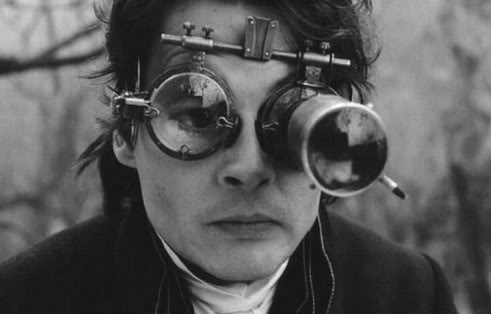
\includegraphics[width=\linewidth]{depp.jpg}
  \caption{Depp's optics (\textit{Sleepy Hollow})}
  \label{fig:marginfig}
\end{marginfigure}

Most optical phenomena can be accounted for using the classical electromagnetic description of light. Complete electromagnetic descriptions of light are, however, often difficult to apply in practice. Geometric optics, treats light as a collection of rays that travel in straight lines and bend when they pass through or reflect from surfaces. Diffraction and interference require a wave model of light and cannot be accounted using geometric optics.

\marginnote[-20pt]{\section{Light Rays}
A light ray is an idealized model of light, obtained by choosing a line that is perpendicular to the wavefronts of the actual light, and that points in the direction of energy flow.  Rays are used to model the propagation of light through an optical system, by dividing the real light field up into discrete rays and tracked through ray tracing.  
\subsection{Ray Angle}
At an interface, ray angles are described relative to the surface normal.}

\section{Refractive Index}
 The refractive index or index of refraction $n$ of a material is a dimensionless number that describes how light propagates through that medium. It is defined as the ratio between the speed of light through vacuum and the speed of light through that material.
 
 $$n=\frac{c}{v}$$

\section{Reflection, Refraction \& Snell's Law}
\begin{marginfigure}[20pt]
  \begin{tikzpicture}[scale=0.65]

    % define coordinates
    \coordinate (O) at (0,0) ;
    \coordinate (A) at (0,4) ;
    \coordinate (B) at (0,-4) ;
    
    % media
    \fill[blue!25!,opacity=.3] (-4,0) rectangle (4,4);
    \fill[blue!60!,opacity=.3] (-4,0) rectangle (4,-4);
    \node[right] at (2,2) {Air, $n_1$};
    \node[left] at (-1.5,-2) {Water, $n_2$};

    % axis
    \draw[dash pattern=on5pt off3pt] (A) -- (B) ;

    % rays
    \draw[red,ultra thick,reverse directed] (O) -- (130:5.2);
     \draw[red,ultra thick, directed] (O)--(-130:-5.2) ;
    \draw[blue,directed,ultra thick] (O) -- (-70:4.24);

    % angles
    \draw (0,1) arc (90:130:1);
     \draw (0,1) arc (90:50:1);
    \draw (0,-1.4) arc (270:290:1.4) ;
    \node[] at (280:1.8)  {$\theta_{2}$};
    \node[] at (110:1.4)  {$\theta_{1}$};
      \node[] at (-110:-1.4)  {$\theta_{1}$};
\end{tikzpicture}
  \caption{Reflection and refraction}
  \label{fig:marginfig}
\end{marginfigure}
\textbf{Reflection} is the change in direction of a wavefront at an interface between two different media so that the wavefront returns into the medium from which it originated. For specular reflection the incident ray angle equals reflected ray angle.
$$\theta_{incidence}=\theta_{reflection} $$
\textbf{Refraction} is the change in direction of propagation of a wave due to a change in its transmission medium.  \textbf{Snell's law} describes the relationship between the angle of the incident ray and that of the refracted ray.

$$n_1\sin\theta_1=n_2\sin\theta_2$$

Snell's law may be derived in various ways.  One way is to match the frequency of the incident and refracted wave at the surface.
\marginnote[-20pt]{\section{Fermat's Principle} 
Fermat's principle states that when light travels between any two points its path is the one that requires the least time.  Snell's law may also be derived from this principle.  In truth it is less of a principle and more of a feature of light and refraction.}
$$f_1=f_2$$
Representing the frequency as a ratio of the velocity and the wavelength yields the following.
$$ \frac{v_1}{\lambda_1}= \frac{v_2}{\lambda_2}$$
Substituting the velocity as the ratio of the speed of light and the index of refraction gives the following.
$$ \frac{c}{n_1\lambda_1}= \frac{c}{n_2\lambda_2}$$
This simplifies further.
$$n_1 \lambda_1 =n_2 \lambda_2 $$
The distance between wave peaks along the interface is $d$.  It must be the same value on both sides of the interface.  Representing the wavelength in terms of $d$ gives the following.
\begin{marginfigure}%
  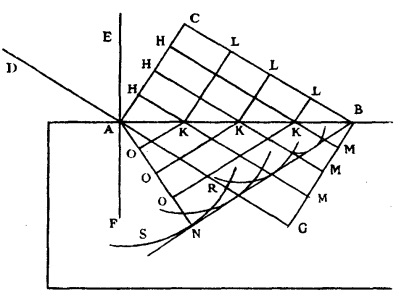
\includegraphics[width=\linewidth]{Huygens_construction.jpg}
  \caption{Huygens' construction}
  \label{fig:marginfig}
\end{marginfigure}
$$n_1 d \sin \theta_1=n_2 d \sin \theta_2$$
Finally cancelling $d$ yields Snell's law. 
$$n_1  \sin \theta_1=n_2  \sin \theta_2$$

\section{Total Internal Reflection}
\begin{marginfigure}[40pt]
  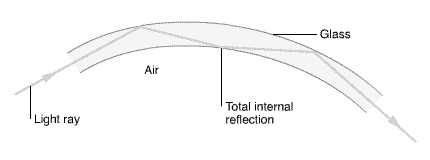
\includegraphics[width=\linewidth]{tir.jpg}
  \caption{Total internal reflection in a fiber optic cable}
  \label{fig:marginfig}
\end{marginfigure}
Total internal reflection is a limiting case of refraction.  In the case of total internal reflection the refracted angle is 90 degrees, namely there is no refracted ray.
$$n_1\sin\theta_c=n_2\sin 90$$
The critical angle for total internal reflection is given as follows.
$$\theta_c=\sin^{-1}\left(\frac{n_2}{n_1}\right)$$
This is possible when light is passing from a medium of higher refractive index to lower refractive index.

\newpage

\section{Dispersion}
\begin{marginfigure}[0pt]
  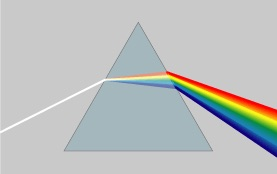
\includegraphics[width=\linewidth]{prism.jpg}
  \caption{Dispersion of white light through a prism}
  \label{fig:marginfig}
\end{marginfigure}

In many wave-propagation media, wave velocity changes with frequency or wavelength of the waves; this is true of light propagation in most transparent substances other than a vacuum. These media are called dispersive. The result is that the angles determined by Snell's law also depend on frequency or wavelength, so that a ray of mixed wavelengths, such as white light, will spread or disperse. Such dispersion of light in glass or water underlies the origin of rainbows and other optical phenomena, in which different wavelengths appear as different colors.  In short, indices of refraction are wavelength dependent.

\subsection{Rainbows}
\begin{marginfigure}[50pt]
  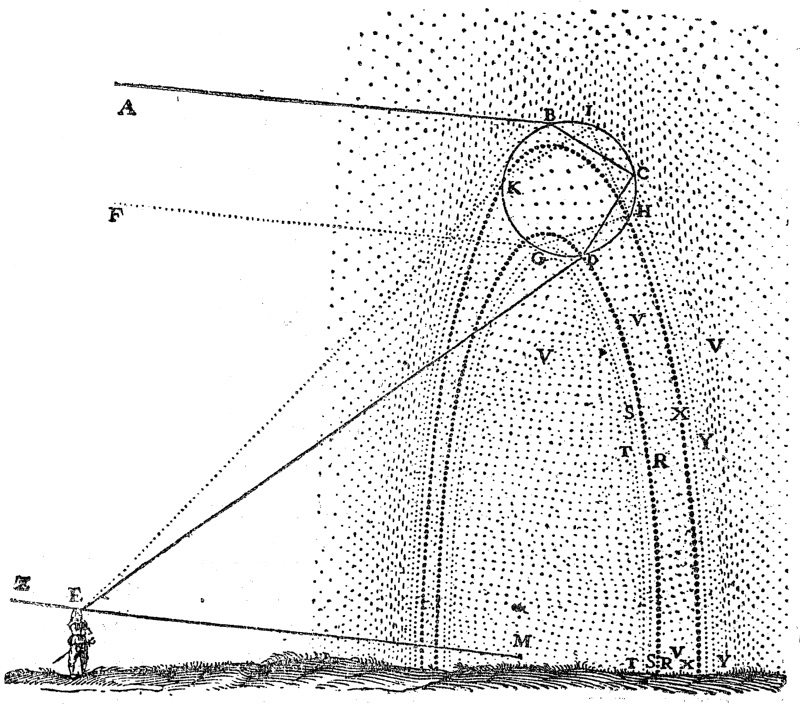
\includegraphics[width=\linewidth]{Descartes_Rainbow.jpg}
  \caption{Descartes diagram of rainbow formation}
  \label{fig:marginfig}
\end{marginfigure}
A rainbow is a meteorological phenomenon that is caused by reflection, refraction and dispersion of light in water droplets resulting in a spectrum of light appearing in the sky. It takes the form of a multicoloured arc. Rainbows caused by sunlight always appear in the section of sky directly opposite the sun.\\
The following diagram shows how rainbows for through light refraction-reflection-refraction interaction with a water droplet.
\vspace{1.5cm}

\begin{figure*}[htbp]
\centering
% Draw an arc denoting an angle using start and delta angles
\newcommand{\drawarcdelta}[4]{
  \draw ($#1+(#2:#4)$) arc[start angle=#2, delta angle=#3, radius=#4];
}

% Draw an arc with label denoting an angle using start and delta angles
\newcommand{\drawlabeledarcdelta}[6]{
  \drawarcdelta{#1}{#2}{#3}{#4}
  \node at ($#1+(#2+#3/2:#6)$) {#5};
}


\begin{tikzpicture}[xscale=-0.8,yscale=0.8,
    ray/.style={decoration={markings,mark=at position .5 with {
      \arrow[>=latex]{>}}},postaction=decorate}
  ]

  % Radius of raindrop
  \pgfmathsetlengthmacro{\r}{3cm}
  % Position where the incoming ray enters the raindrop, as a fraction of
  % the height of the drop.  If 0., the ray will enter in the middle of the
  % drop, if 1., the ray will enter at the top of the drop.
  \pgfmathsetmacro{\f}{.7}

  % Various radii for drawing angle arcs and labels
  \pgfmathsetlengthmacro{\arcradius}{.8cm}
  \pgfmathsetlengthmacro{\dotradius}{.6cm}
  \pgfmathsetlengthmacro{\arclabelradius}{1cm}

  % Calculation of the angle of incidence
  \pgfmathsetmacro{\incidentangle}{asin(\f)}

  % Coordinates of origin and point of entry
  \coordinate (O) at (0, 0);
  \coordinate (A) at (\incidentangle:\r);

  % Draw the drop and the incoming ray, as well as the angle of incidence
  \draw (O) circle (\r);
  \draw[ray] (A  -| \r*3, 0) -- (A);
  \draw[gray] (O) -- ($(O)!1.5!(A)$) node[pos=1.05] {$n$};
  \drawarcdelta{(A)}{0}{\incidentangle}{\arcradius-1pt}
  \drawlabeledarcdelta{(A)}{0}{\incidentangle}{\arcradius+1pt}
    {$i$}{\arclabelradius}

  % For each red and blue ray.  The index of refraction for red light is
  % slightly exaggerated, it should be 1.33.
  \foreach \index/\color in {1.32/red, 1.34/blue} {
    % Calculate angle of refraction
    \pgfmathsetmacro{\refractedangle}{asin(sin(\incidentangle) / \index)}
    % Calculate top angle (at O) in the triangle formed by O, the point of
    % entry, and the point of internal reflection
    \pgfmathsetmacro{\angleindrop}{180 - 2*\refractedangle}

    % Coordinate of point of reflection
    \coordinate (A') at (\incidentangle+\angleindrop:\r);
    % Coordinate of point of exit
    \coordinate (A'') at (\incidentangle+2*\angleindrop:\r);

    \begin{scope}[opacity=.5, color=\color]
      % Draw the light rays
      \draw[ray] (A) -- (A');
      \draw[ray] (A') -- (A'');
      \draw[ray] (A'') -- ($(A'')+(2*\incidentangle+2*\angleindrop:2*\r)$);

      % Draw the normal lines
      \draw (O) -- ($(O)!1.5!(A')$) node[pos=1.05] {$n$};
      \draw (O) -- ($(O)!1.5!(A'')$) node[pos=1.05] {$n$};

      % Draw the arcs and labels
      \drawlabeledarcdelta{(A)}{\incidentangle+180}{-\refractedangle}
        {\arcradius}{$r$}{\arclabelradius}
      \drawarcdelta{(A')}{\incidentangle+\angleindrop+180}{\refractedangle}
        {\arcradius}
      \drawarcdelta{(A')}{\incidentangle+\angleindrop+180}{-\refractedangle}
        {\arcradius}
      \drawarcdelta{(A'')}{\incidentangle+2*\angleindrop+180}{\refractedangle}
        {\arcradius}
    \end{scope}

    % Draw the arcs of the angles of the rays leaving the raindrop.  Note
    % that the angles are identical to the original angle of incidence.
    \drawarcdelta{(A'')}{\incidentangle+2*\angleindrop}{\incidentangle}
      {\arcradius-1pt}
    \drawarcdelta{(A'')}{\incidentangle+2*\angleindrop}{\incidentangle}
      {\arcradius+1pt}
  }

  % Mark the center of the raindrop
  \draw[fill] (O) circle (1.5pt);
\end{tikzpicture}
\caption{Raindrop producing a rainbow}
  \label{fig:GreyScaleSimilarity}
\end{figure*}
\newpage



\section{Geometric Optics}
Geometric optics uses ray tracing to model light. 

\marginnote[-50pt]{
\subsection{Thin Lens Equation}
Light's interaction with thin lenses can be modeled using the thin lens equation.  Here $f$ is the focal length, $d_i$ is the distance from the lens to image and $d_o$ is the distance from the lens to the object.
$$\frac{1}{f}=\frac{1}{d_i}+\frac{1}{d_o}$$
}
\section{Convergent/Convex Lenses (f>0)}
As light rays parallel to the optical axis hit a convergent lens they are scattered to pass through the focus.  The rays converge on the focal point.  Convex lenses are convergent.  \\
\begin{figure*}[htbp]
\centering

\begin{tikzpicture}[scale=0.8]

\filldraw[fill=green!20!white, draw=green!50!black] 
(-0.3,-2.5) -- (0.3,-2.5) arc (-9.148:9.148:15.725) -- (-0.3,2.5) arc (170.852:189.148:15.725);

\draw [color=black!30] (8,-2) -- (8,2);

\draw (-10,0) -- (10,0);
\draw [color=gray] (0,-2.6) -- (0,2.6);

\draw [color=red!50] (-10,1) -- (0,1);
\draw [color=red!50] (-10,2) -- (0,2);
\draw [color=red!50] (-10,-1) -- (0,-1);
\draw [color=red!50] (-10,-2) -- (0,-2);

\draw [color=red!50]  (0,1) -- (10,-1.5);
\draw [color=red!50]  (0,2) -- (10,-3);
\draw [color=red!50] (0,-1) -- (10,1.5);
\draw [color=red!50] (0,-2) -- (10,3);

\fill (4,0) circle (0.1);
\draw (4,0) node [anchor=north,scale=1.5] {$f$};
\fill (8,0) circle (0.1);
\draw (8,0) node [anchor=north,scale=1.5] {$2f$};


\end{tikzpicture}

 \caption{Convergent Lens}
  \label{fig:GreyScaleSimilarity}
\end{figure*}
\marginnote[0pt]{
\subsection{Magnification}
Magnification is the ratio of the height of the focused image $h_i$ to the height of the light emitting object $h_o$.
$$M=\frac{h_i}{h_o}=-\frac{d_i}{d_o}$$}
A light emitting object with a $d_0$ greater that $2f$ will produce an image with a $d_i$ between $f$ and $2f$.  The magnification in this case is negative and has a magnitude which is less than one.
\vspace{2cm}

\begin{figure*}[htbp]
\centering

\begin{tikzpicture}[scale=0.8]

\filldraw[fill=green!20!white, draw=green!50!black] 
(-0.3,-2.5) -- (0.3,-2.5) arc (-9.148:9.148:15.725) -- (-0.3,2.5) arc (170.852:189.148:15.725);

%\draw [color=black!30] (8,-2) -- (8,2);

\draw (-10,0) -- (10,0);
\draw [color=gray] (0,-2.6) -- (0,2.6);


\draw [color=red!50] (-9,2) -- (0,2);
\draw [color=red!50] (-9,2) -- (10,-2.222);
\draw [color=red!50] (-9,2) -- (0,-1.6);
\draw [color=red!50] (0,-1.6) -- (10,-1.6);

\draw [color=red!50]  (0,2) -- (10,-3);


\draw [->, color=blue, line width = 1mm] (-9,0) -- (-9,2);

\draw [->, color=blue, line width = 1mm] (7.2,0) -- (7.2,-1.6);

\fill [color=blue] (-9,0) circle (0.1);
\fill [color=blue] (7.2,0) circle (0.1);


\fill (4,0) circle (0.1);
\draw (4,0) node [anchor=north,scale=1.5] {$f$};
\fill (8,0) circle (0.1);
\draw (8,0) node [anchor=north,scale=1.5] {$2f$};


\fill (-4,0) circle (0.1);
\draw (-4,0) node [anchor=north,scale=1.5] {$f$};
\fill (-8,0) circle (0.1);
\draw (-8,0) node [anchor=north,scale=1.5] {$2f$};
\draw (-9,0) node [anchor=north,scale=1.5] {$d_o$};
\draw (-9,1) node [anchor=east,scale=1.5] {$h_o$};
\draw (7.2,0) node [anchor=south,scale=1.5] {$d_i$};
\draw (7.2,-0.8) node [anchor=east,scale=1.5] {$h_i$};



\end{tikzpicture}

 \caption{$d_0>2f$}
  \label{fig:GreyScaleSimilarity}
\end{figure*}

A light emitting object with a $d_0$ equal $2f$ will produce an image with a $d_i$ equal to $2f$.  The magnification in this case is negative one.
 \newpage

\begin{figure*}[htbp]
\centering

\begin{tikzpicture}[scale=0.8]

\filldraw[fill=green!20!white, draw=green!50!black] 
(-0.3,-2.5) -- (0.3,-2.5) arc (-9.148:9.148:15.725) -- (-0.3,2.5) arc (170.852:189.148:15.725);

%\draw [color=black!30] (8,-2) -- (8,2);

\draw (-10,0) -- (10,0);
\draw [color=gray] (0,-2.6) -- (0,2.6);


\draw [color=red!50] (-8,2) -- (0,2);
\draw [color=red!50] (-8,2) -- (10,-2.5);
\draw [color=red!50] (-8,2) -- (0,-2);
\draw [color=red!50] (0,-2) -- (10,-2);

\draw [color=red!50]  (0,2) -- (10,-3);


\draw [->, color=blue, line width = 1mm] (-8,0) -- (-8,2);

\draw [->, color=blue, line width = 1mm] (8,0) -- (8,-2);

\fill [color=blue] (-8,0) circle (0.1);
\fill [color=blue] (8,0) circle (0.1);


\fill (4,0) circle (0.1);
\draw (4,0) node [anchor=north,scale=1.5] {$f$};

\draw (8,0) node [anchor=south,scale=1.5] {$2f$};


\fill (-4,0) circle (0.1);
\draw (-4,0) node [anchor=north,scale=1.5] {$f$};

\draw (-8,0) node [anchor=north,scale=1.5] {$2f$};
%\draw (-9,0) node [anchor=north,scale=1.5] {$d_o$};
\draw (-8,1) node [anchor=east,scale=1.5] {$h$};
%\draw (8,0) node [anchor=south,scale=1.5] {$d_i$};
\draw (8,-0.8) node [anchor=west,scale=1.5] {$h$};



\end{tikzpicture}

 \caption{$d_0=2f$}
  \label{fig:GreyScaleSimilarity}
\end{figure*}
A light emitting object with a $d_0$ between $2f$ and $f$ will produce an image with a $d_i$ greater than $2f$.  The magnification in this case is negative and has a magnitude which is greater than one.

\begin{figure*}[htbp]
\centering

\begin{tikzpicture}[scale=0.8]

\filldraw[fill=green!20!white, draw=green!50!black] 
(-0.3,-2.5) -- (0.3,-2.5) arc (-9.148:9.148:15.725) -- (-0.3,2.5) arc (170.852:189.148:15.725);

%\draw [color=black!30] (8,-2) -- (8,2);

\draw (-10,0) -- (10,0);
\draw [color=gray] (0,-2.6) -- (0,2.6);


\draw [color=red!50] (-7.2,2) -- (0,2);
\draw [color=red!50] (-7.2,2) -- (10,-2.7777);
\draw [color=red!50] (-7.2,2) -- (0,-2.5);
\draw [color=red!50] (0,-2.5) -- (10,-2.5);

\draw [color=red!50]  (0,2) -- (10,-3);


\draw [->, color=blue, line width = 1mm] (-7.2,0) -- (-7.2,2);

\draw [->, color=blue, line width = 1mm] (9,0) -- (9,-2.5);

\fill [color=blue] (-7.2,0) circle (0.1);
\fill [color=blue] (9,0) circle (0.1);


\fill (4,0) circle (0.1);
\draw (4,0) node [anchor=north,scale=1.5] {$f$};
\fill (8,0) circle (0.1);
\draw (8,0) node [anchor=north,scale=1.5] {$2f$};


\fill (-4,0) circle (0.1);
\draw (-4,0) node [anchor=north,scale=1.5] {$f$};
\fill (-8,0) circle (0.1);
\draw (-8,0) node [anchor=north,scale=1.5] {$2f$};
\draw (-7.2,0) node [anchor=north,scale=1.5] {$d_o$};
\draw (-7.2,1) node [anchor=east,scale=1.5] {$h_o$};
\draw (9,0) node [anchor=south,scale=1.5] {$d_i$};
\draw (9,-1.25) node [anchor=west,scale=1.5] {$h_i$};



\end{tikzpicture}

 \caption{$2f>d_0>f$}
  \label{fig:GreyScaleSimilarity}
\end{figure*}

A light emitting object with a $d_0$ equal to $f$ will not produce an image since the rays transmitted through the lens will be parallel.  The image may be described as existing at infinity.

\begin{figure*}[htbp]
\centering

\begin{tikzpicture}[scale=0.8]

\filldraw[fill=green!20!white, draw=green!50!black] 
(-0.3,-2.5) -- (0.3,-2.5) arc (-9.148:9.148:15.725) -- (-0.3,2.5) arc (170.852:189.148:15.725);

%\draw [color=black!30] (8,-2) -- (8,2);

\draw (-10,0) -- (10,0);
\draw [color=gray] (0,-2.6) -- (0,2.6);


\draw [color=red!50] (-4,2) -- (0,2);
\draw [color=red!50] (-4,2) -- (6,-3);
%\draw [color=red!50] (-7.2,2) -- (0,-2.5);
%\draw [color=red!50] (0,-2.5) -- (10,-2.5);

\draw [color=red!50]  (0,2) -- (10,-3);


\draw [->, color=blue, line width = 1mm] (-4,0) -- (-4,2);

%\draw [->, color=blue, line width = 1mm] (9,0) -- (9,-2.5);


%\fill [color=blue] (9,0) circle (0.1);


\fill (4,0) circle (0.1);
\draw (4,0) node [anchor=north,scale=1.5] {$f$};
\fill (8,0) circle (0.1);
\draw (8,0) node [anchor=north,scale=1.5] {$2f$};


\fill [color=blue] (-4,0) circle (0.1);;
\draw (-4,0) node [anchor=north,scale=1.5] {$f$};
\fill (-8,0) circle (0.1);
\draw (-8,0) node [anchor=north,scale=1.5] {$2f$};
%\draw (-7.2,0) node [anchor=north,scale=1.5] {$d_o$};
%\draw (-7.2,1) node [anchor=east,scale=1.5] {$h_o$};
%\draw (9,0) node [anchor=south,scale=1.5] {$d_i$};
%\draw (9,-1.25) node [anchor=west,scale=1.5] {$h_i$};



\end{tikzpicture}

 \caption{$d_0=f$}
  \label{fig:GreyScaleSimilarity}
\end{figure*}

A light emitting object with a $d_0$ less than $f$ will not produce an image since the rays transmitted through the lens will diverge.  The image may be described as existing with a $d_i$ that is negative.  The image does not exist.  It is virtual.  The magnification is positive and greater than one.

\newpage

\begin{figure*}[htbp]
\centering

\begin{tikzpicture}[scale=0.8]

\filldraw[fill=green!20!white, draw=green!50!black] 
(-0.3,-2.5) -- (0.3,-2.5) arc (-9.148:9.148:15.725) -- (-0.3,2.5) arc (170.852:189.148:15.725);

%\draw [color=black!30] (8,-2) -- (8,2);

\draw (-10,0) -- (10,0);
\draw [color=gray] (0,-2.6) -- (0,2.6);


\draw [color=red!50] (-2,2) -- (0,2);
\draw [color=red!50] (-2,2) -- (2.5,-2.5);



\draw [color=red!50]  (0,2) -- (10,-3);


\draw [->, color=blue, line width = 1mm] (-2,0) -- (-2,2);

\draw [->, dotted, color=blue, line width = 1mm] (-4,0) -- (-4,4);

\fill [color=blue] (-2,0) circle (0.1);
\fill [color=blue] (-4,0) circle (0.1);


\fill (4,0) circle (0.1);
\draw (4,0) node [anchor=north,scale=1.5] {$f$};
\fill (8,0) circle (0.1);
\draw (8,0) node [anchor=north,scale=1.5] {$2f$};



\draw (-4,0) node [anchor=north,scale=1.5] {$f$};
\fill (-8,0) circle (0.1);
\draw (-8,0) node [anchor=north,scale=1.5] {$2f$};
\draw (-2,0) node [anchor=north,scale=1.5] {$f/2$};
\draw (-2,1) node [anchor=east,scale=1.5] {$h$};
%\draw (9,0) node [anchor=south,scale=1.5] {$d_i$};
\draw (-4,2) node [anchor=east,scale=1.5] {$2h$};

\draw [color=red!50,dashed]  (0,2) -- (-4,4);
\draw [color=red!50,dashed]  (-2,2) -- (-4,4);

\end{tikzpicture}

 \caption{$d_0<f$}
  \label{fig:GreyScaleSimilarity}
\end{figure*}


\section{Divergent/Concave Lenses (f<0)}
As light rays parallel to the optical axis hit a divergent lens they are scattered away from the optical axis and do not converge at a point.  Geometrically they diverge as if they come from a point on the other side of the lens.  This point is the focal point of a divergent lens.  The focal length of a divergent lens is negative.  Concave lenses are divergent.

\begin{figure*}[htbp]
\centering

\begin{tikzpicture}[scale=0.7]

\filldraw[fill=green!20!white, draw=green!50!black] 
(-0.3,-2.5) -- (0.3,-2.5) arc (189.148:170.852:15.725) -- (-0.3,2.5) arc (9.148:-9.148:15.725);
\draw [color=black!30] (-8,-2) -- (-8,2);
\draw (-10,0) -- (10,0);
\draw [color=gray] (0,-2.6) -- (0,2.6);

\draw [color=red!50] (-10,1) -- (0,1);
\draw [color=red!50] (-10,2) -- (0,2);
\draw [color=red!50] (-10,-1) -- (0,-1);
\draw [color=red!50] (-10,-2) -- (0,-2);

\draw [color=red!50]  (0,1) -- (10,3.5);
\draw [color=red!50]  (0,2) -- (10,7);
\draw [color=red!50] (0,-1) -- (10,-3.5);
\draw [color=red!50] (0,-2) -- (10,-7);

\draw [color=red!50, dashed]  (0,1) -- (-10,-1.5);
\draw [color=red!50,dashed]  (0,2) -- (-10,-3);
\draw [color=red!50,dashed] (0,-1) -- (-10,1.5);
\draw [color=red!50,dashed] (0,-2) -- (-10,3);

\fill (-4,0) circle (0.1);
\draw (-4,0) node [anchor=north,scale=1.5] {$f$};
\fill (-8,0) circle (0.1);
\draw (-8,0) node [anchor=north,scale=1.5] {$2f$};

\end{tikzpicture}

 \caption{Divergent Lens: parallel lines diverge from focus}
  \label{fig:GreyScaleSimilarity}
\end{figure*}

\newpage
A light emitting object with a $d_0$ greater than $2f$ will not produce an image since the rays transmitted through the lens will diverge.  The image may be described as existing with a $d_i$ that is negative and less than $f$ in absolute value.  The image does not exist.  It is virtual.  The magnification is positive and less than one.

\begin{figure*}[htbp]
\centering

\begin{tikzpicture}[scale=0.7]

\filldraw[fill=green!20!white, draw=green!50!black] 
(-0.3,-2.5) -- (0.3,-2.5) arc (189.148:170.852:15.725) -- (-0.3,2.5) arc (9.148:-9.148:15.725);

%\draw [color=black!30] (8,-2) -- (8,2);

\draw (-10,0) -- (10,0);
\draw [color=gray] (0,-2.6) -- (0,2.6);


\draw [color=red!50] (-9,2) -- (0,2);
\draw [color=red!50] (-9,2) -- (0,0.6153);
\draw [color=red!50] (-9,2) -- (10,-2.222);
\draw [color=red!50]  (0,0.6153) -- (10,0.6153);
\draw [color=gray!50]  (0,0.6153) -- (4,0);
\draw [color=red!50,dashed]  (0,0.6153) -- (-10,0.6153);



\draw [color=red!50,dashed]  (0,2) -- (-10,-3);
\draw [color=red!50,dashed]  (0,2) -- (-10,-3);

\draw [->, color=blue, line width = 1mm] (-9,0) -- (-9,2);

\draw [->, color=blue, dotted, line width = 1mm] (-2.769,0) -- (-2.769,0.6153);

\fill [color=blue] (-9,0) circle (0.1);
\fill [color=blue] (-2.769,0) circle (0.1);


\fill (4,0) circle (0.1);
\draw (4,0) node [anchor=north,scale=1.5] {$f$};
\fill (8,0) circle (0.1);
\draw (8,0) node [anchor=north,scale=1.5] {$2f$};


\fill (-4,0) circle (0.1);
\draw (-4,0) node [anchor=north,scale=1.5] {$f$};
\fill (-8,0) circle (0.1);
\draw (-8,0) node [anchor=north,scale=1.5] {$2f$};
\draw (-9,0) node [anchor=north,scale=1.5] {$d_o$};
\draw (-9,1) node [anchor=east,scale=1.3] {$h_o$};
\draw (-2.769,0) node [anchor=north,scale=1.5] {$d_i$};
\draw (-2.769,0.3077) node [anchor=west,scale=1.3] {$h_i$};

\draw [color=red!50]  (0,2) -- (10,7);

\end{tikzpicture}

 \caption{Convergent Lens: $d_o>2f$}
  \label{fig:GreyScaleSimilarity}
\end{figure*}

In the case where $d_0$ is equal to $2f$ no image is produced since the rays transmitted through the lens will diverge.  The image may be described as existing with a $d_i$ that is negative and two thirds of $f$.  Again the image does not exist, it is virtual.  The magnification is one third.

\begin{figure*}[htbp]
\centering

\begin{tikzpicture}[scale=0.75]

\filldraw[fill=green!20!white, draw=green!50!black] 
(-0.3,-2.5) -- (0.3,-2.5) arc (189.148:170.852:15.725) -- (-0.3,2.5) arc (9.148:-9.148:15.725);

%\draw [color=black!30] (8,-2) -- (8,2);

\draw (-10,0) -- (10,0);
\draw [color=gray] (0,-2.6) -- (0,2.6);


\draw [color=red!50] (-8,2) -- (0,2);
\draw [color=red!50] (-8,2) -- (0,0.6666);
\draw [color=red!50] (-8,2) -- (10,-2.5);
\draw [color=red!50]  (0,0.66666) -- (10,0.666);
\draw [color=gray!50]  (0,0.6666) -- (4,0);
\draw [color=red!50,dashed]  (0,0.66666) -- (-10,0.66666);



\draw [color=red!50,dashed]  (0,2) -- (-10,-3);
\draw [color=red!50,dashed]  (0,2) -- (-10,-3);

\draw [->, color=blue, line width = 1mm] (-8,0) -- (-8,2);

\draw [->, color=blue, dotted,, line width = 1mm] (-2.666,0) -- (-2.66666,0.6153);


\fill [color=blue] (-2.666,0) circle (0.1);


\fill (4,0) circle (0.1);
\draw (4,0) node [anchor=north,scale=1.5] {$f$};
\fill (8,0) circle (0.1);
\draw (8,0) node [anchor=north,scale=1.5] {$2f$};


\fill (-4,0) circle (0.1);
\draw (-4,0) node [anchor=north,scale=1.5] {$f$};
\fill [color=blue] (-8,0) circle (0.1);
\draw (-8,0) node [anchor=north,scale=1.5] {$2f$};

\draw (-8,1) node [anchor=east,scale=1.3] {$h$};
%\draw (-2.666,0) node [anchor=north,scale=1.1] {$(2f)/3$};
%\draw (-2.6666,0.3333) node [anchor=west,scale=1.1] {$h/3$};

\draw [color=red!50]  (0,2) -- (10,7);

\end{tikzpicture}

 \caption{Convergent Lens:  $d_o=2f$}
  \label{fig:GreyScaleSimilarity}
\end{figure*}

\newpage

In the case where $d_0$ is equal to $f$ no image is produced since the rays transmitted through the lens will diverge.  The image may be described as existing with a $d_i$ that is negative and two half of $f$.  Again the image does not exist, it is virtual.  The magnification is one half.

\begin{figure*}[htbp]
\centering

\begin{tikzpicture}[scale=0.75]

\filldraw[fill=green!20!white, draw=green!50!black] 
(-0.3,-2.5) -- (0.3,-2.5) arc (189.148:170.852:15.725) -- (-0.3,2.5) arc (9.148:-9.148:15.725);

%\draw [color=black!30] (8,-2) -- (8,2);

\draw (-10,0) -- (10,0);
\draw [color=gray] (0,-2.6) -- (0,2.6);


\draw [color=red!50] (-4,2) -- (0,2);
\draw [color=red!50] (-4,2) -- (0,1);
\draw [color=red!50] (-4,2) -- (10,-5);
\draw [color=red!50]  (0,1) -- (10,1);
\draw [color=gray!50]  (0,1) -- (4,0);
\draw [color=red!50,dashed]  (0,1) -- (-10,1);



\draw [color=red!50,dashed]  (0,2) -- (-10,-3);
\draw [color=red!50,dashed]  (0,2) -- (-10,-3);

\draw [->, color=blue, line width = 1mm] (-4,0) -- (-4,2);

\draw [->, color=blue, dashed, line width = 1mm] (-2,0) -- (-2,1);


\fill [color=blue] (-2,0) circle (0.1);


\fill (4,0) circle (0.1);
\draw (4,0) node [anchor=north,scale=1.5] {$f$};
\fill (8,0) circle (0.1);
\draw (8,0) node [anchor=north,scale=1.5] {$2f$};


\fill [color=blue] (-4,0) circle (0.1);
\draw (-4,0) node [anchor=north,scale=1.5] {$f$};
\fill [color=black] (-8,0) circle (0.1);
\draw (-8,0) node [anchor=north,scale=1.5] {$2f$};

\draw (-4,1) node [anchor=east,scale=1.3] {$h$};
%\draw (-2.666,0) node [anchor=north,scale=1.1] {$f/2$};
%\draw (-2.6666,0.3333) node [anchor=west,scale=1.1] {$h/2$};

\draw [color=red!50]  (0,2) -- (10,7);

\end{tikzpicture}

 \caption{Convergent Lens: $d_o=f$}
  \label{fig:GreyScaleSimilarity}
\end{figure*}

\section{Mirrors}
Mirrors work the same way lenses do except light is reflected rather than transmitted.  Convergent mirrors are concave while divergent lenses are convex.  

\section{Characterizing Images}
\begin{description}
\item[real/virtual] Real images can be focused on a plane and occur when light converges.  Virtual images cannot be focused on a plane and occur when light diverges.
\item[upright/inverted] Upright images are right-side-up versions of the object and occur for $M>0$ while inverted images are up-side-down versions of the object and occur for $M<0$.
\item[enlarged/reduced] Enlarged images are bigger versions of the object and occur for $|M|>0$ while reduced images are smaller versions of the object and occur for $|M|<0$.
\end{description}

\newpage


\section{Huygens Principle}
\begin{marginfigure}[0pt]
  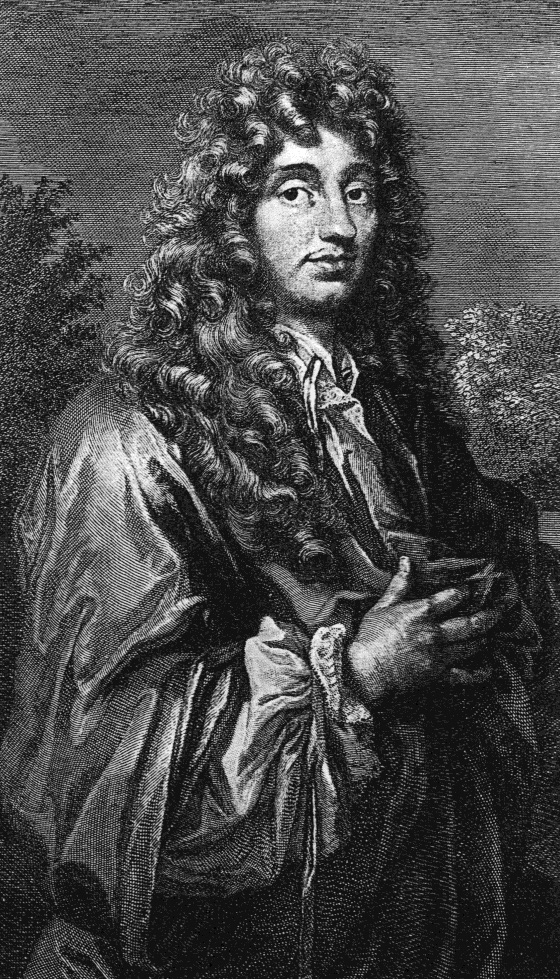
\includegraphics[width=\linewidth]{Christiaan_Huygens.jpg}
  \caption{Christiaan Huygens had sausage fingers}
  \label{fig:marginfig}
\end{marginfigure}
Huygens principle states that every point which a luminous disturbance reaches becomes a source of a spherical wave.  In other words, all points bombarded by waves become point sources for waves.


\section{Interference}
Light wave interference requires the following criteria.
\begin{itemize}
  \item Sources must be coherent, namely maintain a constant phase relative to one another.
  \item Sources must be monochromatic, namely be of a single wavelength.
  \item Superposition must apply
\end{itemize}

\section{Double Slit Experiment}
\begin{marginfigure}[30pt]
  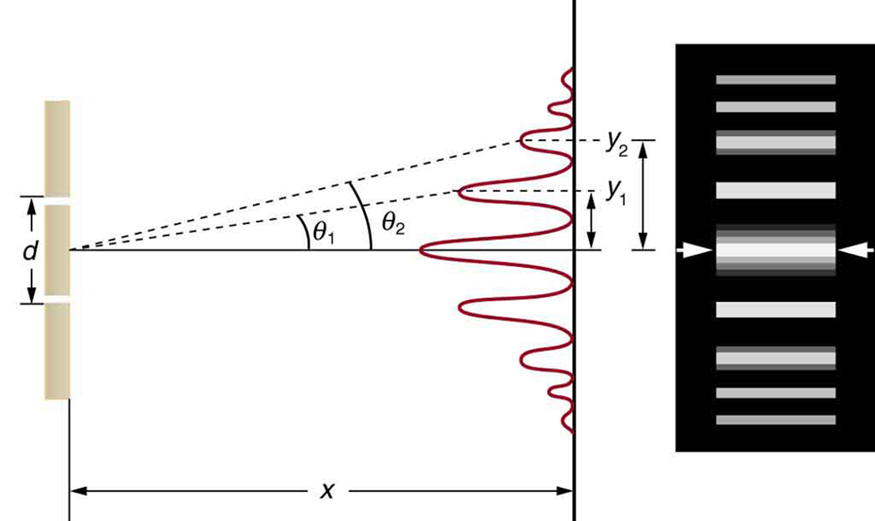
\includegraphics[width=\linewidth]{diffraction.jpg}
  \caption{Two slit diffraction}
  \label{fig:marginfig}
\end{marginfigure}
Conducted by Young 1801.  Consider two slits separated by a distance $d$.  Light interferes on a plane distance $L$ away.  For $L>>d$ we may use parallel ray approximation to determine path difference $\delta$.  
\begin{marginfigure}[10pt]
  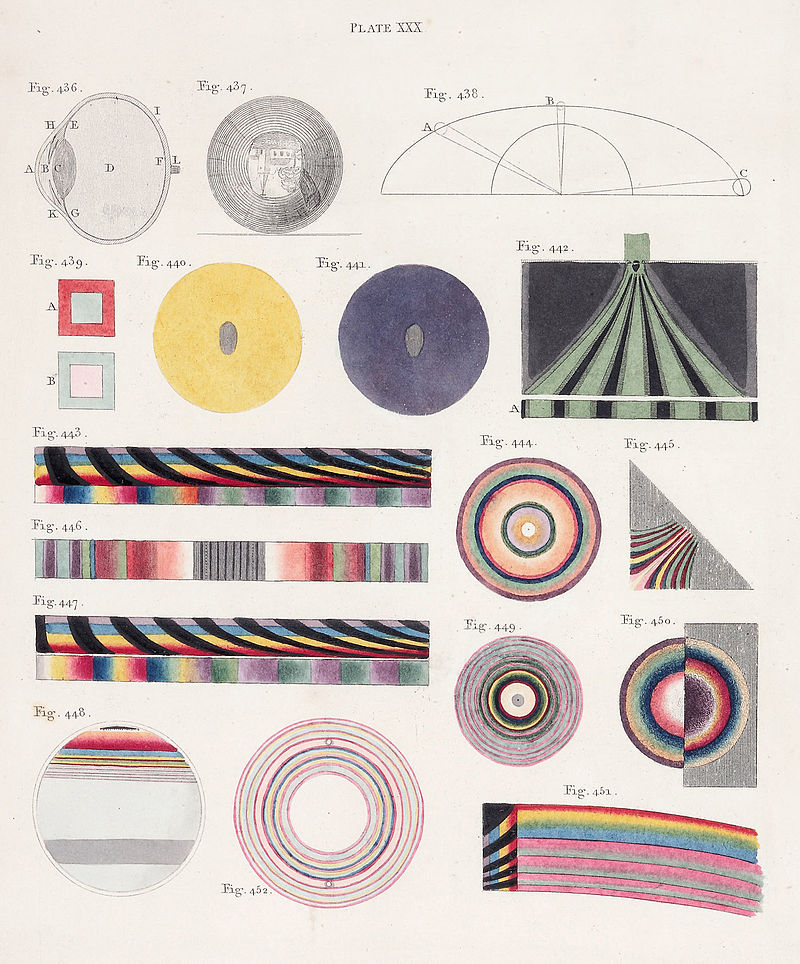
\includegraphics[width=\linewidth]{Young_Plate.jpg}
  \caption{Plate from Thomas Young's 1807 \textit{Lectures on Natural Philosophy and the Mechanical Arts}}
  \label{fig:marginfig}
\end{marginfigure}
$$\delta=r_2-r_1=d\sin\theta$$
Constructive interference associated with bright spots on the plane.
$$d\sin\theta=N\lambda$$
Similar phenomena for a diffraction grating where $d$ is the distance between slits.
 
 \subsection{Intensity}
 Phase difference is related to the path difference and wavelength.
 $$\phi=\frac{2\pi}{\lambda}\delta=\frac{2\pi}{\lambda}d\sin\theta$$
 The total electric field is the sum of the two components of electric field. 
 $$E_T=E_1+E_2=E_0\cos(\omega t)+E_0\cos(\omega t+\phi)=2E_0\cos(\phi/2)\cos(\omega t +\phi/2)$$
 Then relating the average intensity to the average electric field squared removes the time dependence and yields the following. 
 $$I_{avg}=I_0\cos^2\left(\frac{\pi d \sin \theta}{\lambda}\right)$$
 
  \vspace{1cm}
 
 \section{Reflection Phase Change}
 An electromagnetic wave undergoes a phase change of 180 degrees upon reflection at an interface with a medium medium of higher refractive index than the one in which the wave is traveling.  (reflection off a window)
 

 
 \section{Thin Film Interference}
 
 Consider a thin film of refractive index $n$ and thickness $l$.  An electromagnetic wave in air hits the interface, part of the wave is reflected with a 180 degree phase change and part is transmitted into the film.  The transmitted component reflects off the other side of the film and is transmitted bad through the original interface to recombine with the reflected component.
 \begin{marginfigure}[-40pt]
  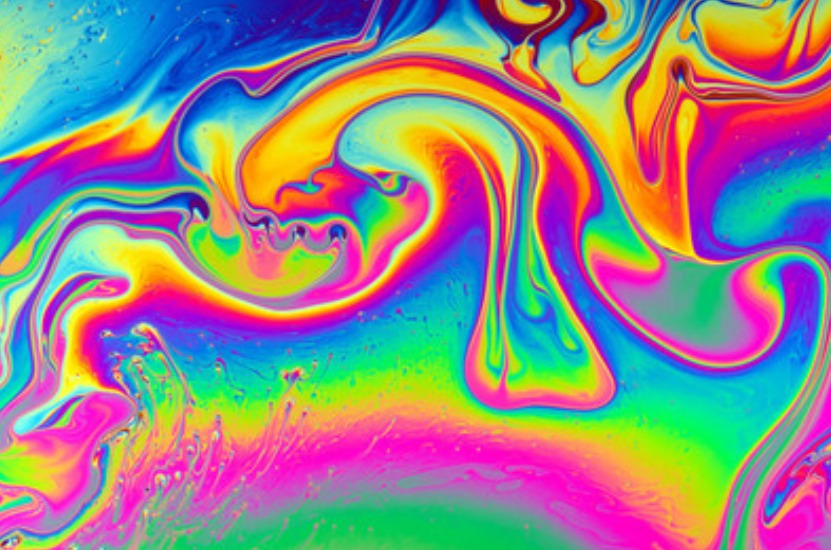
\includegraphics[width=\linewidth]{oil_rainbow.jpg}
  \caption{Thin film of oil}
  \label{fig:marginfig}
\end{marginfigure}

\marginnote[30pt]{
\subsection{Iridescence}
Iridescence caused by thin-film interference is a commonly observed phenomenon in nature, being found in a variety of plants and animals. One of the first known studies of this phenomenon was conducted by Robert Hooke in 1665. In \textit{Micrographia}, Hooke postulated that the iridescence in peacock feathers was caused by thin, alternating layers of plate and air. In 1704, Isaac Newton stated in his book, \textit{Opticks}, that the iridescence in a peacock feather was due to the fact that the transparent layers in the feather were so thin. In 1801, Thomas Young provided the first explanation of constructive and destructive interference.}

 \subsection{Constructive Interference}
 For constructive interference to occur the path difference must be equivalent an integer multiple of wavelengths plus half a wavelength.  This is due to the fact that there is a reflection which takes place.  This is equivalent to a half-phase shift.
 $$2l=\left(N+\frac{1}{2}\right)\frac{\lambda}{n}$$
 Constructive interference is desired for reflective coatings.
  \subsection{Destructive Interference}
  For destructive interference to occur the path difference must be an integer multiple of waves.  The integer multiple of wave will produce destructive interference because there is an additional half-phase shift due to the reflection
 $$2l=N\frac{\lambda}{n}$$
 Destructive interference is desired for anti-glare coatings.
 
